\documentclass[border=4pt]{standalone}
\usepackage{tikz}
\usetikzlibrary{arrows.meta}

\begin{document}
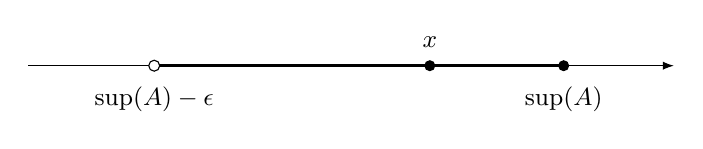
\begin{tikzpicture}[x=1cm, y=1cm, font=\small]

    \draw[-{Latex[length=4pt]}] (0,0) -- (8.2,0);
    \draw[very thick] (1.6,0) -- (6.8,0);
    \node[circle, draw, fill=white, inner sep=1.4pt] at (1.6,0) {};
    \fill (5.1,0) circle (2pt);
    \fill (6.8,0) circle (2pt);
    \node[above=3pt] at (5.1,0) {$x$};
    \node[below=4pt] at (1.6,0) {$\sup(A)-\epsilon$};
    \node[below=4pt] at (6.8,0) {$\sup(A)$};

\end{tikzpicture}
\end{document}
